\documentclass[tikz,border=10pt]{standalone}
\usepackage{pgfplots}
\usetikzlibrary{arrows.meta}

\begin{document}
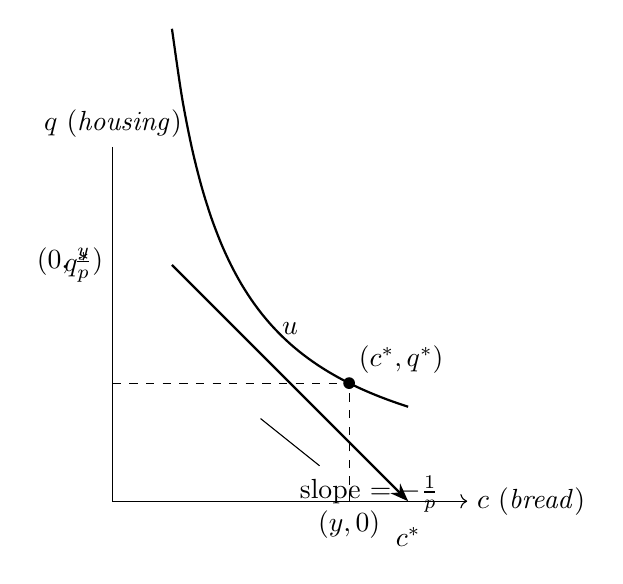
\begin{tikzpicture}[scale=1.5, every node/.style={scale=1}]
  % Axes
  \draw[->] (0,3) node[above] {$q$ (\textit{housing})} -- (0,0) -- (3,0) node[right] {$c$ (\textit{bread})};

  % Indifference curve
  \draw[thick, domain=0.5:2.5, smooth, variable=\x] plot ({\x}, {2/\x});
  \node at (1.5,1.33) [above] {$u$};

  % Budget constraint
  \draw[thick, -Stealth] (0.5,2) -- (2.5,0);
  \node at (2.5,-0.3) {$c^*$};
  \node at (-0.3,2) {$q^*$};
  \draw[dashed] (2,0) -- (2,1);
  \draw[dashed] (0,1) -- (2,1);
  \node at (2,1) [circle,fill,inner sep=1.5pt]{};
  \node at (2,1) [above right] {$(c^*,q^*)$};

  % Slope
  \draw (1.25,0.7) -- (1.75,0.3);
  \node at (1.5,0.3) [below right] {slope $= -\frac{1}{p}$};

  % Point labels
  \node at (0,2) [left] {$(0, \frac{y}{p})$};
  \node at (2,0) [below] {$(y,0)$};

\end{tikzpicture}
\end{document}
